\chapter{Réalisation}

\section{Introduction}
L'objectif de cette partie est de donner aux lecteurs de ce rapport un aperçu détaillé des différentes interfaces du système de gestion de l'apprentissage (LMS) de United Associates, développé en partenariat avec DEG\&PARTNERS. Ce chapitre présente les fonctionnalités offertes aux différents acteurs du système, notamment les collaborateurs, les gestionnaires et les formateurs.

\section{Présentation des interfaces}

\subsection{Interface principale du tableau de bord}
L'interface principale du LMS constitue le point d'entrée central pour tous les utilisateurs. Elle présente une vue d'ensemble personnalisée des activités de formation et des objectifs temporels.

\begin{figure}[H]
    \centering
    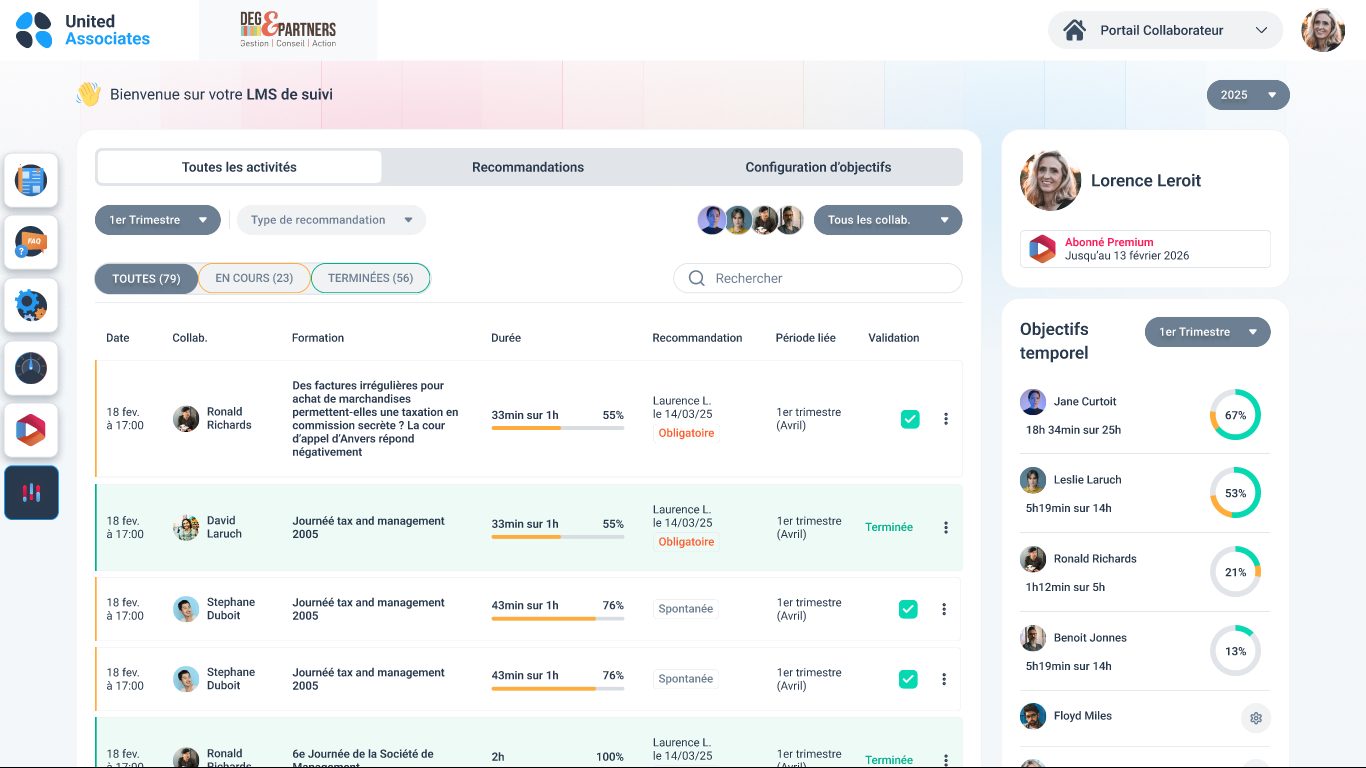
\includegraphics[width=\textwidth]{realisation/toutactivite.png}
    \caption{Interface principale du LMS}
    \label{fig:interface_principale}
\end{figure}

Cette interface comprend plusieurs sections principales :
\begin{itemize}
    \item \textbf{Barre de navigation} : Permettant l'accès aux différentes fonctionnalités (Toutes les activités, Recommandations, Configuration d'objectifs)
    \item \textbf{Panneau d'activités} : Affichant les formations en cours, terminées et à venir avec leurs statuts respectifs
    \item \textbf{Section objectifs temporels} : Présentant les progrès individuels des collaborateurs avec des indicateurs visuels
\end{itemize}

\subsection{Interface de gestion des recommandations}
Cette interface permet aux utilisateurs de consulter et gérer les recommandations de formation personnalisées.

\begin{figure}[H]
    \centering
    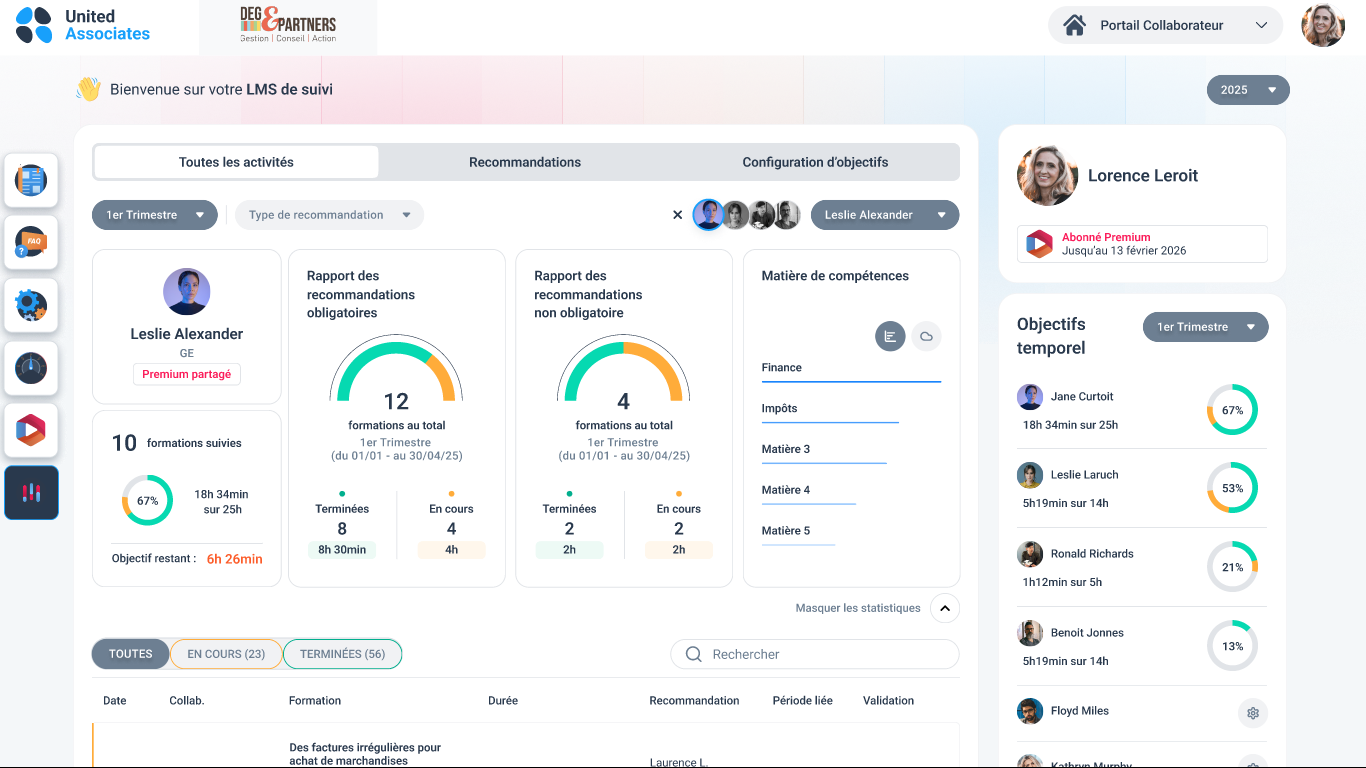
\includegraphics[width=\textwidth]{realisation/user.png}    
    \caption{Interface des recommandations d'un collaborateur}
    \label{fig:interface_recommandations}

\end{figure}
\begin{figure}[H]
    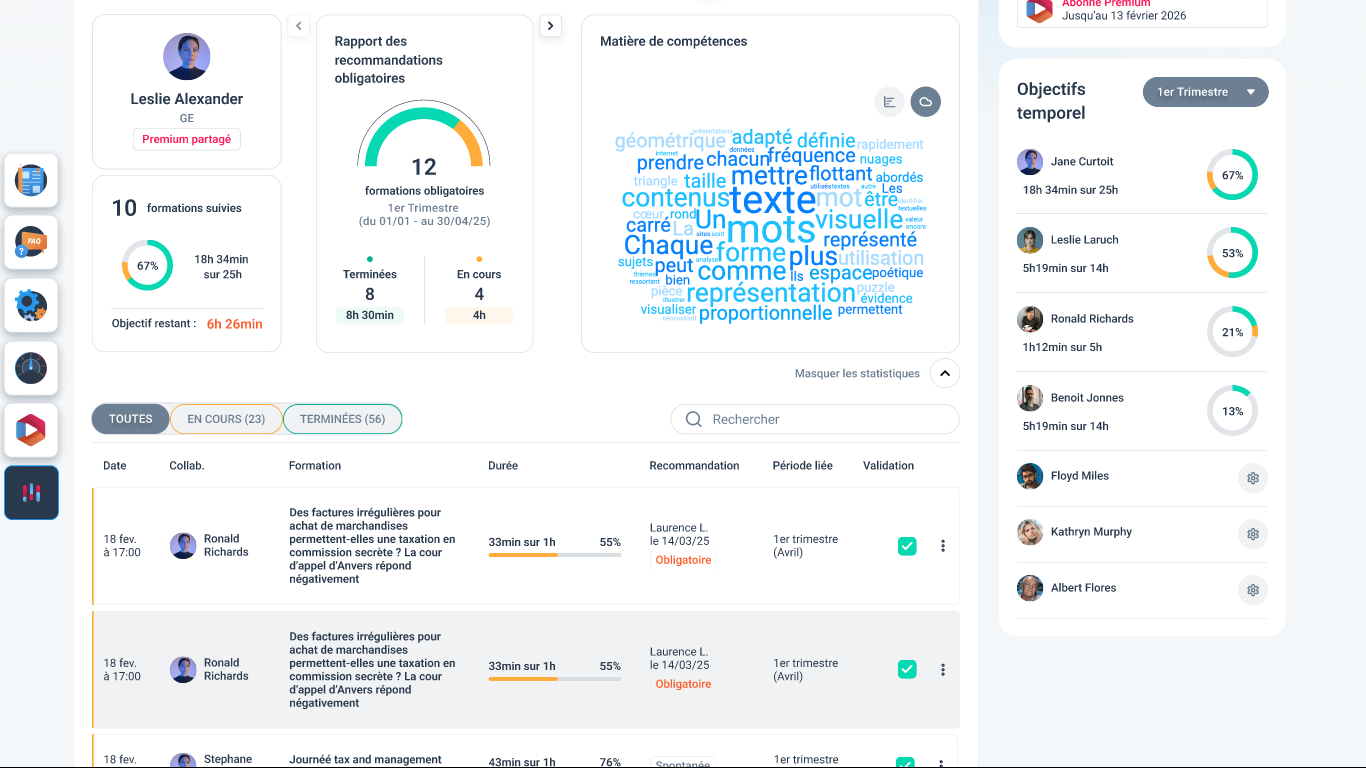
\includegraphics[width=\textwidth]{realisation/userwithmot.png}
    \caption{Interface des recommandations}
    \label{fig:interface_recommandations}
\end{figure}

L'interface des recommandations offre :
\begin{itemize}
    \item \textbf{Profil utilisateur} : Affichage des informations personnelles et du statut Premium
    \item \textbf{Rapport des recommandations obligatoires} : Visualisation graphique des formations obligatoires avec indicateurs de progression
    \item \textbf{Matière de compétences} : Nuage de mots interactif présentant les domaines de compétences
    \item \textbf{Historique des formations} : Liste détaillée des formations suivies et à suivre
\end{itemize}

\subsection{Interface de création d'objectifs}
Cette interface permet aux gestionnaires de définir et configurer les objectifs de formation pour leurs équipes.

\begin{figure}[H]
    \centering
    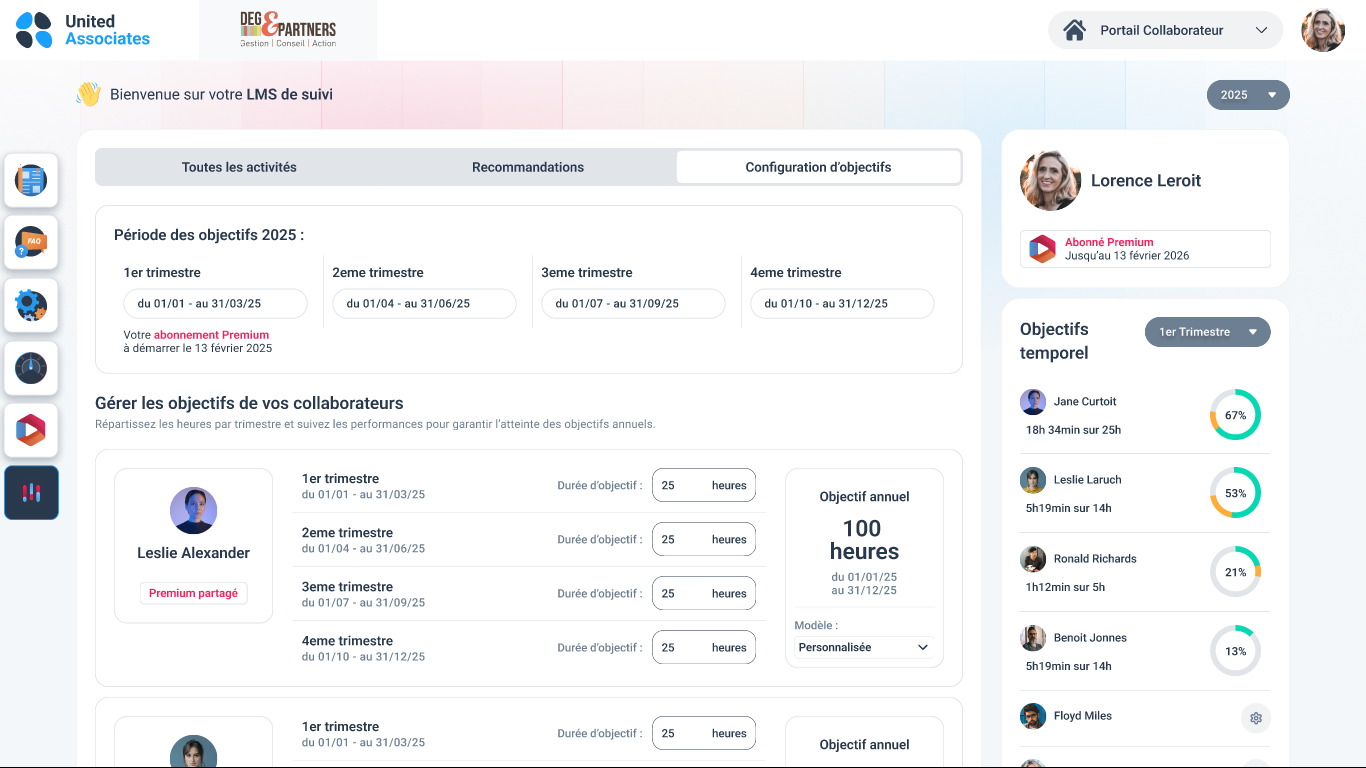
\includegraphics[width=\textwidth]{realisation/goal.png}
    \caption{Interface de création d'objectifs}
    \label{fig:creation_objectifs}
\end{figure}

Les fonctionnalités incluent :
\begin{itemize}
    \item \textbf{Création de modèles d'objectifs} : Définition de titres et paramètres personnalisés
    \item \textbf{Gestion par trimestre} : Répartition des objectifs sur l'année avec durées spécifiques
    \item \textbf{Objectifs annuels} : Configuration d'objectifs globaux avec suivi temporel
\end{itemize}

\subsection{Interface de configuration des objectifs collaborateurs}
Cette interface permet une gestion détaillée des objectifs individuels des collaborateurs.

\begin{figure}[H]
    \centering
    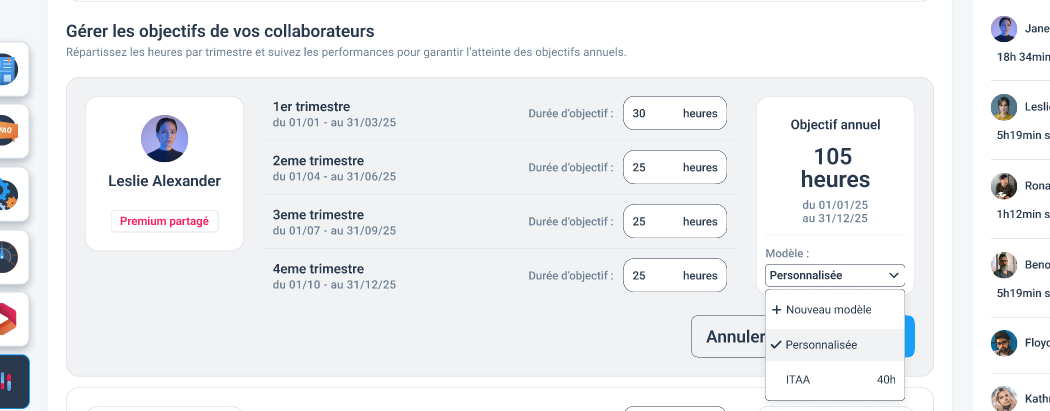
\includegraphics[width=\textwidth]{realisation/model.png}
    \caption{Interface de configuration des objectifs}
    \label{fig:config_objectifs}
\end{figure}

Elle comprend :
\begin{itemize}
    \item \textbf{Gestion par période} : Visualisation des objectifs par trimestre avec dates précises
    \item \textbf{Objectifs personnalisés} : Configuration d'heures de formation par collaborateur
    \item \textbf{Suivi des performances} : Affichage des objectifs annuels et du progrès réalisé
\end{itemize}

\subsection{Interface de recommandation de formations}
Cette interface facilite la recherche et l'assignation de formations aux collaborateurs.

\begin{figure}[H]
    \centering
    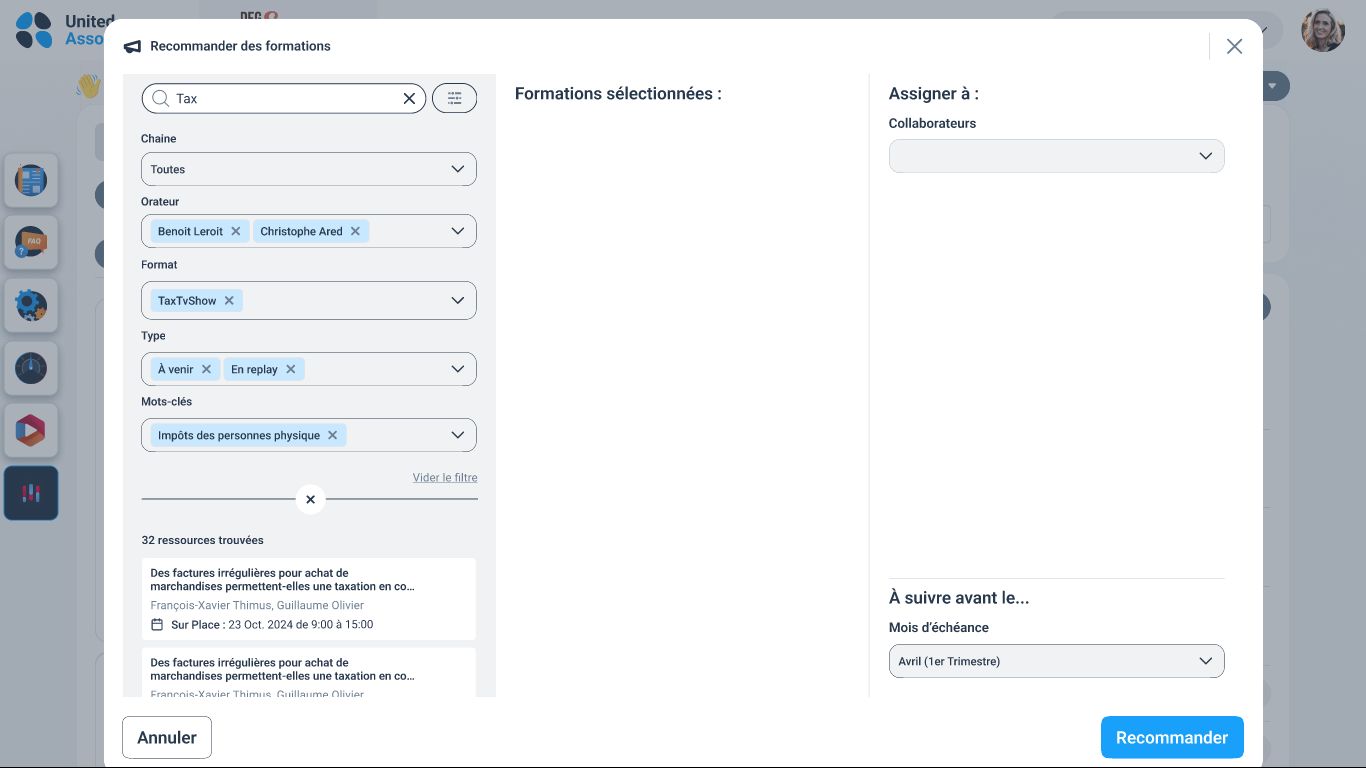
\includegraphics[width=\textwidth]{realisation/cherch.png}
    \caption{Interface de recherche de formations}
    \label{fig:recherche_formations}
\end{figure}

Les fonctionnalités principales sont :
\begin{itemize}
    \item \textbf{Moteur de recherche} : Recherche par mots-clés dans le catalogue de formations
    \item \textbf{Filtrage avancé} : Sélection de formations spécifiques par critères
    \item \textbf{Assignation multiple} : Possibilité d'assigner des formations à plusieurs collaborateurs
    \item \textbf{Planification} : Configuration des échéances et modalités de formation
\end{itemize}

\subsection{Interface de sélection et assignation}
Cette interface permet une gestion fine de l'assignation des formations aux équipes.

\begin{figure}[H]
    \centering
    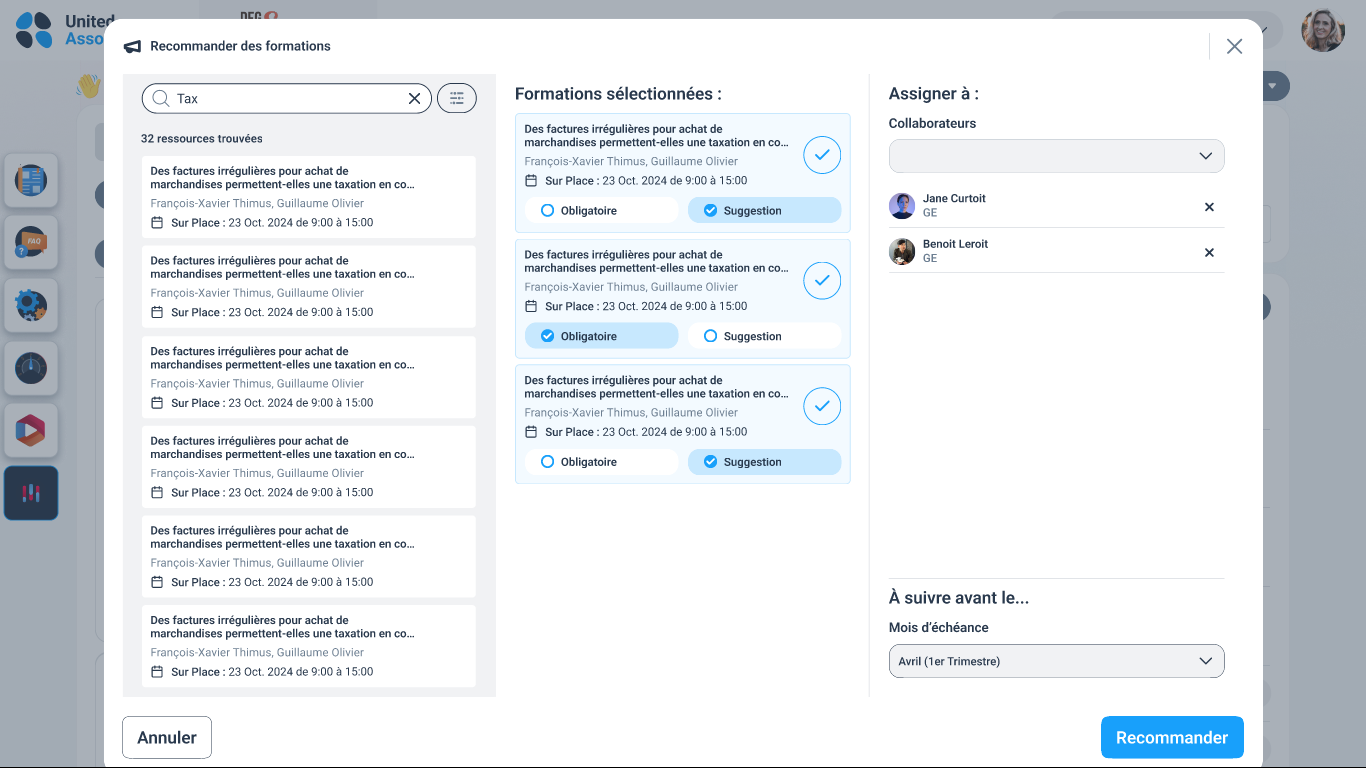
\includegraphics[width=\textwidth]{realisation/selection.png}
    \caption{Interface de sélection des formations}
    \label{fig:selection_formations}
\end{figure}

Elle offre :
\begin{itemize}
    \item \textbf{Sélection multiple} : Choix de plusieurs formations simultanément
    \item \textbf{Types de recommandations} : Distinction entre formations obligatoires et suggestions
    \item \textbf{Gestion des collaborateurs} : Assignation ciblée par collaborateur
    \item \textbf{Planification temporelle} : Configuration des dates d'échéance
\end{itemize}

\subsection{Interface de suivi des recommandations}
Cette interface présente le suivi des formations recommandées et leur statut d'avancement.

\begin{figure}[H]
    \centering
    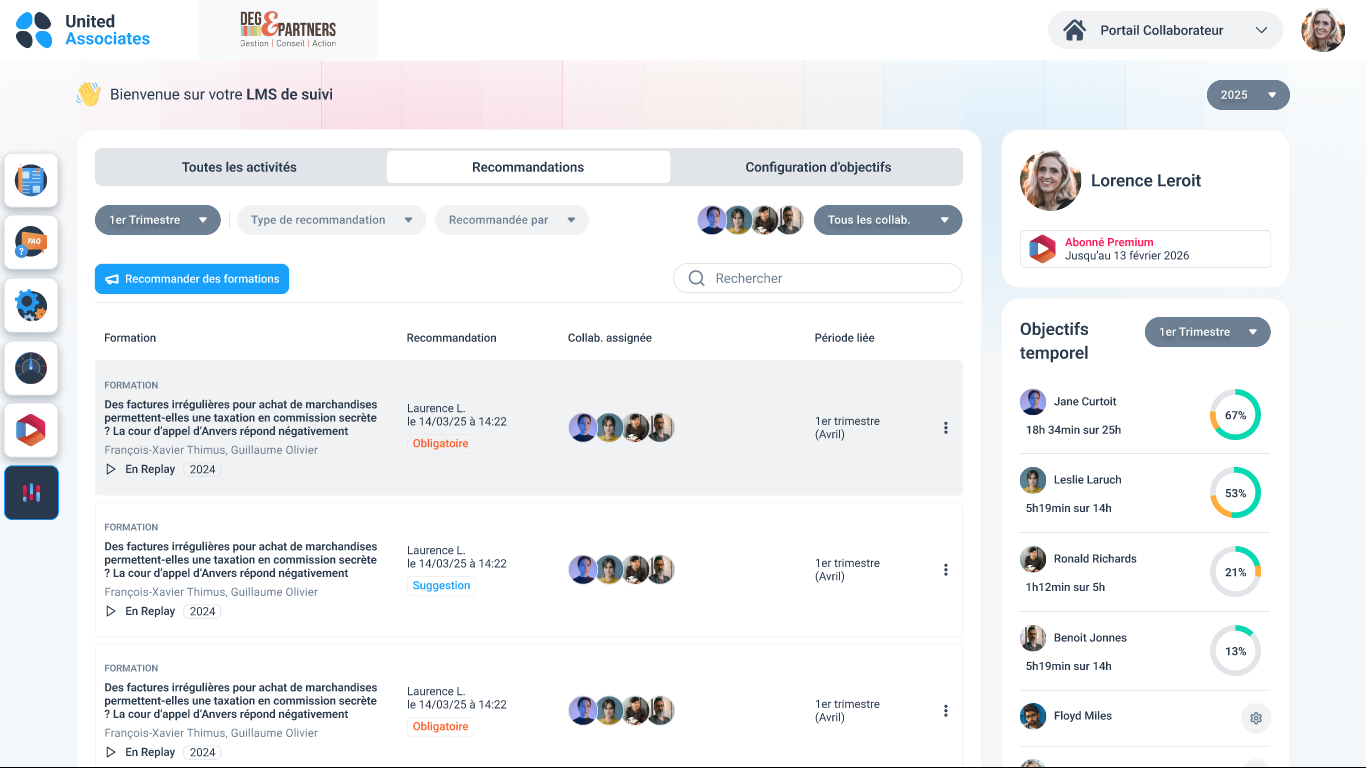
\includegraphics[width=\textwidth]{realisation/recomendation.png}
    \caption{Interface de suivi des recommandations}
    \label{fig:suivi_recommandations}
\end{figure}

Les éléments clés comprennent :
\begin{itemize}
    \item \textbf{Tableau de suivi} : Vue d'ensemble des formations assignées
    \item \textbf{Statuts de recommandation} : Distinction entre obligations et suggestions
    \item \textbf{Suivi par collaborateur} : Visualisation des formations par équipe
    \item \textbf{Indicateurs de progression} : Suivi des échéances et de l'avancement
\end{itemize}

\section{Fonctionnalités transversales}

\subsection{Système de notification}
Le système intègre un mécanisme de notifications pour informer les utilisateurs des échéances, nouvelles formations et objectifs à atteindre.

\subsection{Tableaux de bord personnalisés}
Chaque utilisateur dispose d'un tableau de bord adapté à son rôle (collaborateur, gestionnaire, formateur) avec des métriques pertinentes.

\subsection{Système de reporting}
Des rapports détaillés permettent le suivi des performances individuelles et collectives, facilitant la prise de décision managériale.
\section{Planification et suivi du projet}

\subsection{Diagramme de Gantt réel}
Le diagramme de Gantt ci-dessous présente la planification réelle du projet de développement du LMS de United Associates, montrant les différentes phases de réalisation, les jalons importants et l'état d'avancement des tâches sur la période de février à juillet 2025.

\begin{figure}[H]
    \centering
    
\includegraphics[width=\textwidth]{gantt_reel.png}
    \caption{Diagramme de Gantt réel du projet LMS}
    \label{fig:gantt_reel}
\end{figure}
Ce diagramme illustre :
\begin{itemize}
    \item \textbf{Phases de développement} : Répartition temporelle des différentes étapes du projet
    \item \textbf{Jalons critiques} : Points de contrôle et livrables importants marqués par des losanges
    \item \textbf{Progression réelle} : Comparaison entre la planification initiale et l'avancement effectif
    \item \textbf{Tâches parallèles} : Identification des activités menées simultanément
    \item \textbf{Dépendances} : Relations entre les différentes tâches du projet
\end{itemize}

L'analyse de ce diagramme révèle que le projet a globalement respecté les échéances prévues, avec quelques ajustements mineurs dans la planification pour optimiser les ressources et la qualité des livrables.
\section{Conclusion}
Ce chapitre a présenté les principales interfaces LMS, illustrant la richesse fonctionnelle de la plateforme. L'ensemble des interfaces développées offre une expérience utilisateur complète, allant de la gestion des objectifs individuels au suivi global des formations, en passant par un système de recommandations personnalisées. Le diagramme de Gantt réel témoigne du respect de la planification et de la bonne gestion temporelle du projet. Cette architecture modulaire permet une adaptation flexible aux besoins spécifiques de chaque organisation tout en maintenant une cohérence ergonomique et fonctionnelle.